\chapter{Graph Colouring}

\tikzset{vtx/.style={circle,fill=black,inner sep=1.6pt}}

\section{Colourings and the chromatic number}

\begin{definition}[$k$-colouring]
A \emph{$k$-colouring} of a graph $G$ is a function $c : V(G) \to \{1, \dots, k\}$ such that
$c(u) \ne c(v)$ whenever $uv \in E(G)$. $G$ is \emph{$k$-colourable} if it has a $k$-colouring.
The \emph{chromatic number} $\chi(G)$ is the least $k$ for which $G$ is $k$-colourable.
\end{definition}

Each colour class $c^{-1}(i)$ is an \emph{independent set} (no two vertices adjacent), so a
$k$-colouring is the same as a partition of $V(G)$ into $k$ independent sets.

\begin{example}
\begin{itemize}
  \item $\chi(G) = 1$ iff $G$ has no edges.
  \item $\chi(K_n) = n$: all vertices are pairwise adjacent, so they need distinct colours.
  \item $\chi(C_n) = 2$ for $n$ even and $3$ for $n$ odd.
  \item $\chi(Q_n) = 2$ for $n \ge 1$.
\end{itemize}
\end{example}

\begin{theorem}
$G$ is $2$-colourable if and only if $G$ is bipartite, if and only if $G$ has no odd cycle.
\end{theorem}
\begin{proof}
A $2$-colouring is exactly a bipartition (the two colour classes). The second equivalence was
proved in the chapter on trees.
\end{proof}

So deciding $\chi(G) \le 2$ is easy (BFS). By contrast, deciding whether $\chi(G) \le 3$ is
NP-complete; no efficient algorithm is known.

\section{Lower bounds}

\begin{proposition}
If $H$ is a subgraph of $G$ then $\chi(H) \le \chi(G)$. In particular, if $G$ contains $K_r$ as
a subgraph (a \emph{clique} of size $r$) then $\chi(G) \ge r$.
\end{proposition}

\begin{proposition}
If $\alpha(G)$ is the size of a largest independent set of $G$ and $G$ has $p$ vertices, then
$\chi(G) \ge p/\alpha(G)$.
\end{proposition}
\begin{proof}
In a $k$-colouring each of the $k$ colour classes has at most $\alpha(G)$ vertices, so
$p \le k\,\alpha(G)$.
\end{proof}

\begin{example}
For $C_5$, $\alpha = 2$, so $\chi \ge 5/2$, i.e.\ $\chi \ge 3$, even though $C_5$ contains no
triangle. The clique bound is not always tight.
\end{example}

\begin{center}
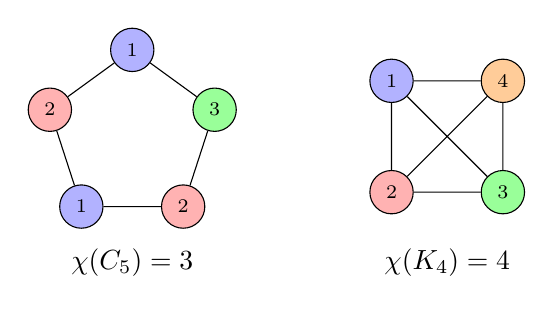
\begin{tikzpicture}[cv/.style={circle,draw,minimum size=0.55cm,inner sep=0pt,font=\scriptsize}]
  \foreach \i/\c/\col in {1/1/blue!30,2/2/red!30,3/1/blue!30,4/2/red!30,5/3/green!40} {
    \node[cv,fill=\col] (c\i) at ({90+72*(\i-1)}:1.1) {$\c$};
  }
  \draw (c1)--(c2)--(c3)--(c4)--(c5)--(c1);
  \node at (0,-1.6) {$\chi(C_5) = 3$};
  \begin{scope}[xshift=4cm]
    \foreach \i/\col in {1/blue!30,2/red!30,3/green!40,4/orange!40} {
      \node[cv,fill=\col] (k\i) at ({90*\i+45}:1) {$\i$};
    }
    \draw (k1)--(k2)--(k3)--(k4)--(k1)--(k3) (k2)--(k4);
    \node at (0,-1.6) {$\chi(K_4) = 4$};
  \end{scope}
\end{tikzpicture}
\end{center}
In the $3$-colouring of $C_5$ the colour classes are $\{\text{top}, \text{lower left}\}$,
$\{\text{upper left}, \text{lower right}\}$ and the single remaining vertex: at most
$\alpha(C_5) = 2$ vertices each.

\section{Upper bounds: greedy colouring}

\begin{important}[Greedy colouring]
Order the vertices $v_1, \dots, v_p$. For $i = 1, \dots, p$, give $v_i$ the smallest colour not
already used on a neighbour $v_j$ with $j < i$.
\end{important}

\begin{theorem}
If $\Delta(G)$ is the maximum degree of $G$, then $\chi(G)\le\Delta(G)+1$.
\end{theorem}
\begin{proof}
In greedy colouring, when $v_i$ is coloured at most $\deg(v_i) \le \Delta$ of its neighbours are
already coloured, so one of the colours $1, \dots, \Delta + 1$ is free.
\end{proof}

The bound is attained by complete graphs and odd cycles, and these are the only connected
examples:

\begin{theorem}[Brooks, statement only]
If $G$ is connected and is neither a complete graph nor an odd cycle, then $\chi(G)\le\Delta(G)$.
\end{theorem}

\begin{important}[Pitfall]
Greedy colouring depends heavily on the order. For the path $v_1v_3v_4v_2$ (edges $v_1v_3$,
$v_3v_4$, $v_4v_2$) in the order $v_1, v_2, v_3, v_4$: $v_1 \gets 1$, $v_2 \gets 1$, $v_3 \gets 2$,
$v_4 \gets 3$. Three colours for a bipartite graph! Some ordering always gives an optimal colouring,
but finding it is hard.
\end{important}

\begin{center}
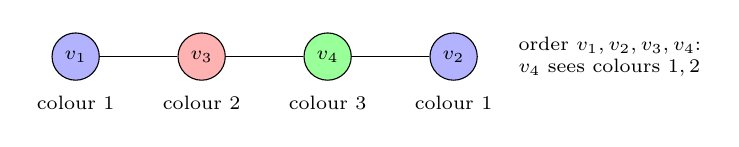
\begin{tikzpicture}[cv/.style={circle,draw,minimum size=0.6cm,inner sep=0pt,font=\scriptsize}]
  \node[cv,fill=blue!30] (1) at (0,0) {$v_1$};
  \node[cv,fill=red!30] (3) at (1.6,0) {$v_3$};
  \node[cv,fill=green!40] (4) at (3.2,0) {$v_4$};
  \node[cv,fill=blue!30] (2) at (4.8,0) {$v_2$};
  \draw (1)--(3)--(4)--(2);
  \foreach \n/\c in {1/1,3/2,4/3,2/1} \node[below=2pt,font=\scriptsize] at (\n.south) {colour \c};
  \node[font=\scriptsize,align=left,right] at (5.5,0) {order $v_1,v_2,v_3,v_4$:\\$v_4$ sees colours $1,2$};
\end{tikzpicture}
\end{center}

A useful refinement: if $G$ has a vertex of degree at most $k$ in every subgraph (a
\emph{$k$-degenerate} graph), then ordering the vertices by repeatedly removing a vertex of
minimum degree (and colouring in reverse order) shows $\chi(G) \le k + 1$. Planar graphs are
$5$-degenerate, which is exactly the six colour theorem argument.

\section{Example: the Petersen graph}

The Petersen graph $P$ (outer $5$-cycle $o_1\cdots o_5$, inner pentagram $n_1n_3n_5n_2n_4$, spokes
$o_in_i$) contains $C_5$, so $\chi(P) \ge 3$. A $3$-colouring:
\[
o_1, o_2, o_3, o_4, o_5 \mapsto 1, 2, 1, 2, 3,\qquad
n_1, n_2, n_3, n_4, n_5 \mapsto 2, 3, 3, 1, 1.
\]
Check the spokes: $(1,2), (2,3), (1,3), (2,1), (3,1)$, all different. Check the pentagram edges
$n_1n_3$ $(2,3)$, $n_3n_5$ $(3,1)$, $n_5n_2$ $(1,3)$, $n_2n_4$ $(3,1)$, $n_4n_1$ $(1,2)$, all
different. The outer cycle uses $1,2,1,2,3$ around, and $o_5o_1$ is $(3,1)$. So $\chi(P) = 3$.

\begin{center}
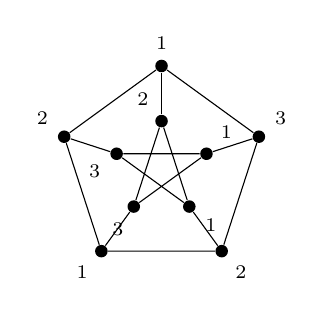
\begin{tikzpicture}[lab/.style={font=\scriptsize}]
  \foreach \i/\c in {1/1,2/2,3/1,4/2,5/3} {
    \node[vtx,label={[lab]{90+72*(\i-1)}:$\c$}] (o\i) at ({90+72*(\i-1)}:1.3) {};
  }
  \foreach \i/\c in {1/2,2/3,3/3,4/1,5/1} {
    \node[vtx,label={[lab]{90+72*(\i-1)+30}:$\c$}] (n\i) at ({90+72*(\i-1)}:0.6) {};
    \draw (o\i)--(n\i);
  }
  \draw (o1)--(o2)--(o3)--(o4)--(o5)--(o1);
  \draw (n1)--(n3)--(n5)--(n2)--(n4)--(n1);
\end{tikzpicture}
\end{center}

\section{Applications}

\begin{example}[Exam scheduling]
Make a vertex for each exam, with an edge between two exams that share a student. A colouring
assigns time slots so that no student has two exams at once, and $\chi(G)$ is the minimum number
of slots.
\end{example}

\begin{example}[Map colouring]
Given a map of countries, make a vertex for each country and join countries sharing a border.
The resulting graph is planar (it is the \emph{dual} of the map), so by the four colour theorem
every map can be coloured with four colours so that neighbouring countries differ.
\end{example}

\section{Edge colouring}

\begin{definition}[Edge colouring]
A \emph{$k$-edge-colouring} assigns colours to edges so that edges sharing an end get different
colours. The least such $k$ is the \emph{edge-chromatic number} $\chi'(G)$.
\end{definition}

Each colour class is a matching (see the next chapter), and clearly $\chi'(G) \ge \Delta(G)$.

\begin{theorem}[Vizing, statement only]
$\Delta(G) \le \chi'(G) \le \Delta(G) + 1$ for every graph $G$.
\end{theorem}

\begin{theorem}[K\"onig, statement only]
If $G$ is bipartite then $\chi'(G) = \Delta(G)$.
\end{theorem}

\begin{example}
$\chi'(C_5) = 3$: each colour class is a matching of $C_5$ with at most $2$ edges, and there are
$5$ edges. $\chi'(K_4) = 3$: the three perfect matchings $\{12,34\},\{13,24\},\{14,23\}$
partition the edges.
\end{example}

\begin{center}
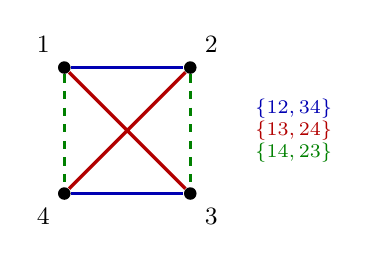
\begin{tikzpicture}[every label/.style={font=\small}]
  \node[vtx,label=above left:$1$] (1) at (0,1.6) {};
  \node[vtx,label=above right:$2$] (2) at (1.6,1.6) {};
  \node[vtx,label=below right:$3$] (3) at (1.6,0) {};
  \node[vtx,label=below left:$4$] (4) at (0,0) {};
  \draw[very thick,blue!70!black] (1)--(2) (3)--(4);
  \draw[very thick,red!70!black] (1)--(3) (2)--(4);
  \draw[very thick,green!50!black,dashed] (1)--(4) (2)--(3);
  \node[font=\scriptsize,align=left,right] at (2.3,0.8) {{\color{blue!70!black}$\{12,34\}$}\\{\color{red!70!black}$\{13,24\}$}\\{\color{green!50!black}$\{14,23\}$}};
\end{tikzpicture}
\end{center}

\section{Summary}
\begin{itemize}
  \item $\chi(G)$: least $k$ with a proper $k$-colouring; colour classes are independent sets.
  \item $\chi\le2$ iff bipartite iff no odd cycles; $\chi(K_n) = n$.
  \item Lower bounds: cliques, $p/\alpha(G)$. Upper bounds: greedy gives $\Delta+1$; Brooks gives
        $\Delta$ except for complete graphs and odd cycles.
  \item Planar graphs: $\chi \le 4$. Edge colouring: $\chi' \in\{\Delta, \Delta+1\}$, and $\chi'=\Delta$
        for bipartite graphs.
\end{itemize}
